\section{Chamber Construction}
\label{construction}

\subsection{Construction Overview}

The three chamber types (called ``regions'', with ``Region 1'' abbreviated as 
``R1'', etc.)  share the same basic design elements simply
scaled up in size by a factor of 1.5 for R2 relative to R1 and a factor
of 2 between R3 and R1. Each chamber is a solid trapezoid in shape, with  
a pair of wire-supporting endplates that bear both the load of the 
wire tensions and the weight of all associated hardware. A representative 
chamber is shown in Fig.~\ref{chamber-exploded}, with the component parts indicated.
This particular drawing is of a R1 chamber, but all chambers have the
same basic parts.

%%%%%%%%%%%%%%%%%%%%%% Figure : generic chamber sketch %%%%%%%%%%%%%%%%%%%%%%
\begin{figure}[htpb]   
\vspace{10cm}
\begin{picture}(35,35)
\put(-70,0)
{\hbox{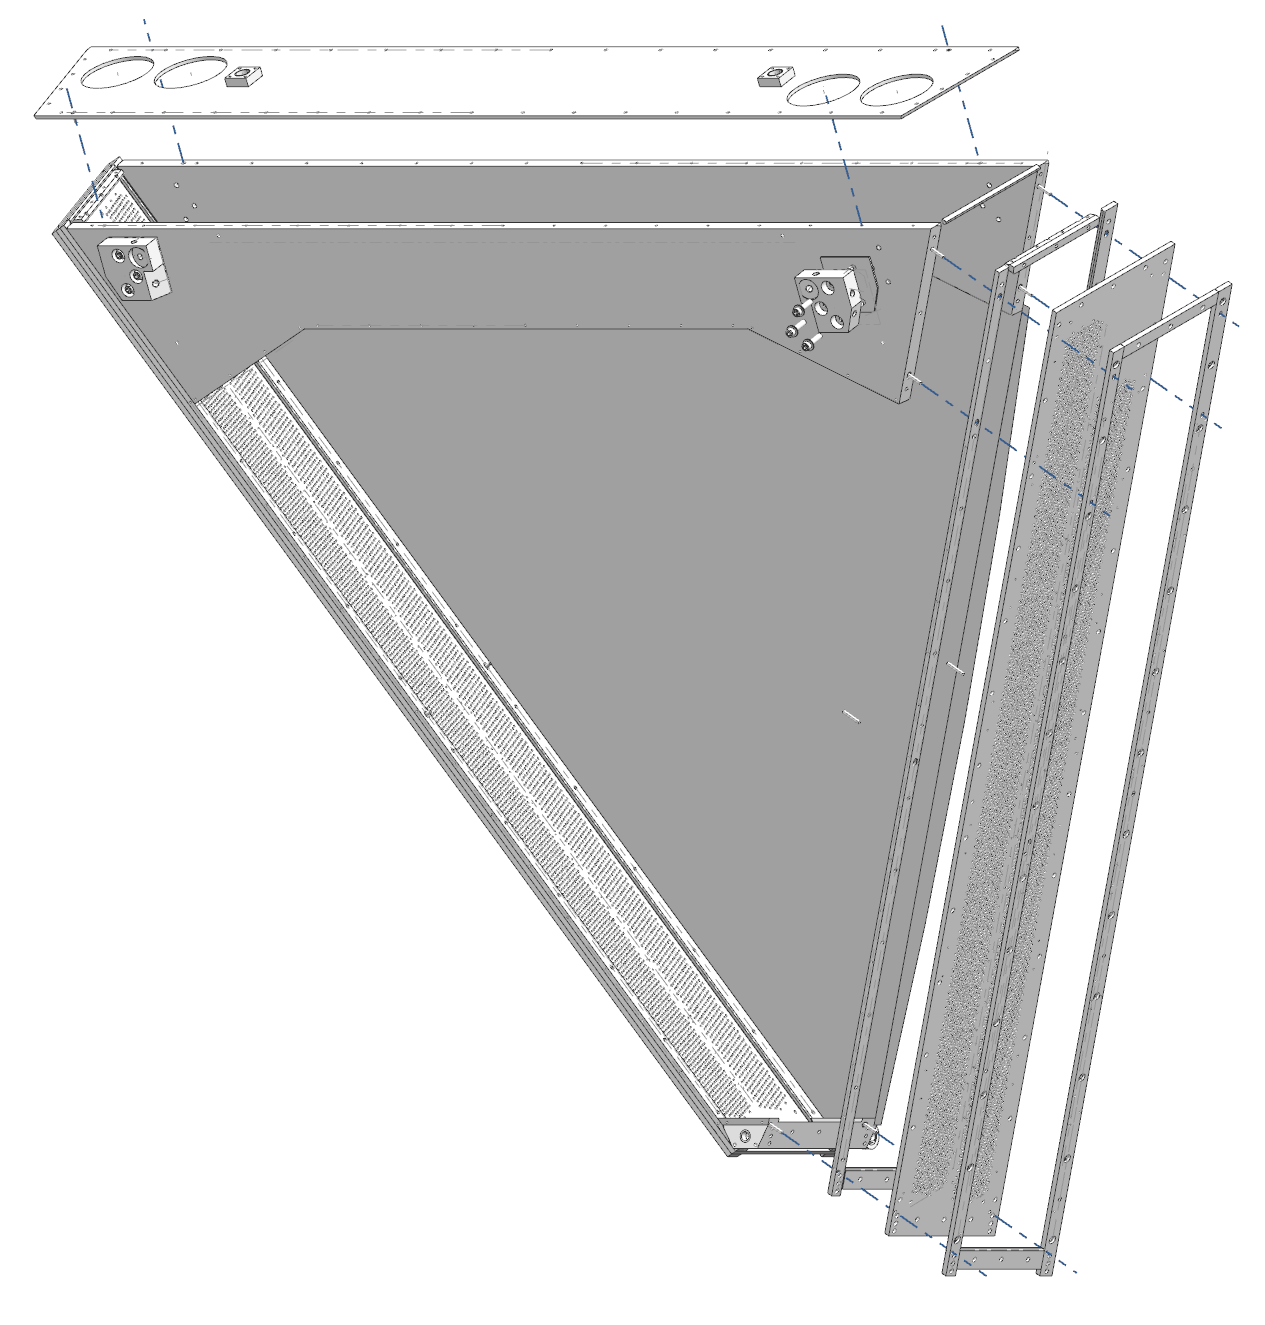
\includegraphics[width=0.9\columnwidth,natwidth=610,natheight=642]{img/chamber-exploded.png}}}
\end{picture}
\caption{\small{Assembly of a typical drift-chamber
(here a R1 sector) highlighting the common component parts.}}
\label{chamber-exploded}
\end{figure}   
%%%%%%%%%%%%%%%%%%%%%%%%%%%%%%%%%%%%%%%%%%%%%%%%%%%%%%%%%%%%%%%

The chamber bodies were constructed from accurately machined plates
(2 endplates, a ``nose-plate'' and a ``back-plate'').
The endplates themselves were an assembly of a main plate with precision-drilled
holes to which we bolted and glued stiffener bars.  In the case of
R1 the main plate was aluminum and the stiffener bars were stainless steel;
for R2 the main plates were non-conducting Stesalit material and the bars stainless steel, and for R3
the main plates were themselves an assembly of two thin steel plates with a foam interior.
No additional stiffener bars were used for R3.

At the radially outward end of each chamber, a thick ``back-plate'' was 
employed to maintain the relative 
alignment of the endplates, to stiffen the chamber against bending moments, 
and to provide a place to attach gas seals and fittings. At the radially inward 
end of each chamber, the endplates were connected together via a small joining 
piece called the ``nose-plate''.  The hardware fabrication and placement 
was of critical importance to the dimensional accuracy of the chambers.

We used many of the same construction materials and procedures as we did
in the previous CLAS chambers.  Please see the previous NIM article \cite{dc12-nim} 
for these details.  For the reader's convenience, we repeat some of descriptions
in this article.

\subsection{Construction Materials}
\label{materials}

To insure a long working life for the chambers, care was taken to 
specify that all materials in contact with the gas volume were clean and ``chamber 
safe'' as defined in Ref.~\cite{kadyk}.  As previously, all construction was carried out in 
Class-10000 or better clean rooms.

The drift-chamber bodies were made primarily of aluminum (R1), Stesalit (an epoxy-fiberglass composite) (R2),
or steel-clad structural foam (R3).  The aluminum and steel parts were 
manufactured with machine oils and, as before, were subsequently cleaned with  
Micro-laboratory detergent from the Cole-Parmer Instrument Company.  The 
Stesalit endplates were machined without any lubricating oils.  Immediately 
prior to chamber assembly all parts were cleaned with detergent, then rinsed with
deionized water and alcohol.  As before, the 
wire feedthroughs and crimp pins were cleaned in an ultrasonic bath 
with detergent and then rinsed in a second ultrasonic bath with deionized water.

It is important to avoid any outgassing into the chamber.  We used Shell Epon resin 826 mixed with Versamid 140, and 
Scotchweld varieties 210 and 2216 for chamber assembly and gluing of feedthroughs.  These mixtures have been 
studied extensively and found not to outgas significantly~\cite{nasa}.

As before, the on-chamber gas tubing is mainly stainless steel, with some
nylon tubing used in the gas manifolds.  Special care was taken during
all steps of construction and testing to ensure that no oils or
silicones contacted any of the chamber materials.

\subsection{Chamber Body Construction}

The construction of the chamber bodies consisted of 3 main stages:
\begin{itemize}
\item receipt, inspection, and cleaning of parts,
\item assembly of the main drilled plate and stiffener bars into a complete endplate,
followed by insertion and gluing of the feedthroughs into the pre-drilled holes 
in the main plate, and 
\item over-all assembly of the endplates and nose- and back-plates to make
a chamber ``box''.
\end{itemize}

\subsubsection{Inspection and Cleaning}

After a visual inspection, we first cleaned the endplates and structural 
frame using a low residue laboratory degreasing solution and water rinse.
We then performed a final cleaning using an ultrasonic bath of a laboratory-grade detergent solution.  
After two hours we rinsed with de-ionized water and then sprayed 
with methanol to aid drying.
We cleaned the feedthroughs and other small parts with a similar procedure.
In addition, the injection-molded parts were specified to be free of silicon 
mold releases.
 
\subsubsection{Endplate and Chamber Body Assembly}

We assenbled the endplates on a table in the cleanroom.  The various parts,
the pre-drilled main plate and the various stiffener bars, were pinned
and glued into place.  Once the endplate assembly was finished,
we inserted and glued the feedthroughs into each hole.  We took special care 
to use the minimal amount of glue required to provide a solid gas 
seal in order to prevent glue contamination inside the detector. 

The feedthroughs are an assembly of a metal trumpet fitted into an injection-molded 
plastic feedthrough.  The metal trumpets were produced on a screw machine, and 
delivered to the injection molding factory.
As with the original CLAS chambers we specified the use of
``Noryl'' plastic reinforced with glass beads to make it stiffer.
It is important to not that the surface conductivity
of this glass-bead loaded composite is little affected by room humidities
as high as 60\%, in contrast to similar plastic strengthened
with microscopic glass strands which performed poorly in high-voltage stand-off
tests in humid conditions.  

Because our chamber endplates are not parallel, but oriented at
\approx 60^{\circ} with respect to each other, the wire position is determined
by the feedthrough's trumpet's concentricity and placement and not by
the concentricity or inner radius of the crimp pin; see Fig.~\ref{dc-corner}.

This allowed us to design the crimp pin to maximize crimp reliability
and ease of use by using soft copper with a large enough inner diameter
to be used for stringing all types of wire: sense, field and guard.
Using a thick-walled copper pin ensured a good crimp through a range of gap settings~\cite{sbc}.
Having a single type of crimper required fewer re-calibrations, the soft
copper made more secure crimps and the larger inner radius made
stringing easier.

Once the endplates were assembled with feedthroughs in place, 
we assembled the chamber box from the
endplates, nose-plate, and back-plate using a variety of special-purpose
fixtures.  With the box held in its final configuration, the parts were bolted
and glued into place using the special glues mentioned in Section~\ref{materials}.
We used precision pinning extensively to achieve high dimensional accuracy.

\subsection{Wire Choice}

Our ``thin endplate'' design required minimizing wire tensions and
thus the diameter of the wire.  The real key to reducing wire tension is to
make the field wires (which are much larger than the sense wires) as 
thin as possible and to make them out of low-density metal.  

In general, designers have chosen very small diameter sense wires because they
require lower operating voltages.
The sense wire choice for all of our chambers, supplied by the Luma
Sweden Company, is 30-$\mu$m diameter gold-plated tungsten.  
The previous CLAS drift chambers used 20-$\mu$m diameter wire for the
sense wires.  We decided to use the thicker 30-$\mu$m wire because it is 
significantly tougher, making it easier to handle without
accidental kinking and less likely to break.

As before, Tungsten was chosen because of its durability, 
and we specified gold-plating because it is chemically inert.  

We chose 80-$\mu$m gold-plated Cu-Be wire for our field wire and
140-$\mu$m gold-plated Cu-Be wire for our guard wires; both supplied
by Little Falls Alloys. Cu-Be wire is very tough, is easily plated, and resists
``flaking'' of the gold plating. 
Minimizing the diameter for the field wire is important because it means that they 
could be strung at lower tension than a thicker wire for the same gravitational sag.  
This minimizes the forces on the endplates that we wanted to keep as 
thin as possible to maximize the solid-angle of the sensitive area of
the chambers.

The 80-$\mu$m diameter was chosen because it is the smallest possible choice
that will not initiate cathode emission at the surface.
We designed for a  gas gain of a few times 
10$^4$; see Section~\ref{operating-voltage} for further discussion of this. 
Under this condition, the electric field at the surface of the sense 
wires is $\approx$200~kV/cm and the surface field at the field wire
surface is less than 50~kV/cm, and this will minimize 
conditions that could cause unwanted cathode emissions and a noisy chamber.  

We note that our choice violated the ``20~kV/cm rule'', the conventional wisdom that
a surface field greater than 20~kV/cm on the cathode wire would lead to 
a noisy chamber. Our own studies showed that there was no cathode emission below
50~kV/cm from any wire with good surface finish~\cite{cathode-emission} .  Each batch
of wire was evaluated with our test device~\cite{patent} to ensure that at operating field 
values there was no emission.  

\subsubsection{Wire Tensions}

A basic principle of our drift chamber design is that each drift cell is a perfect hexagon.
We used this geometrical constraint to determine the hole placement in the endplates.
This geometrical design assumed that wires are straight lines.  Of course, real wires
sag across the wire span due to gravity.  To keep our perfect hexagonally shaped cells,
we tensioned our three types of wires (sense, field, and guard) such that they
{\bf sagged equally} under their gravitational loads.

Our 30~$\mu$m tungsten sense wires, 80~$\mu$m Cu-Be field wires, and 140~$\mu$m Cu-Be guard
wires had linear densities of 0.014, 0.042, and 0.129~g/m, respectively.  To sag equally
under gravity, they were strung at 20, 62, and 190~g of tension, respectively.
In each chamber there were 12 rows of 112 sense wires, 28 rows of 112 field wires,
and 4 rows of 112 guard wires for a total wire tension of 306~kg.
This caused some bowing of our thin endplates. This bowing and the sagging
of the wires themselves is discussed in the Section~\ref{geom_distortions} on geometrical distortions.

\subsection{Chamber Wire Stringing}


Because all of the chambers have the same shape, differing only in
size and some materials, we strung them all using the same basic method.
They were gravity-strung using a similar methodology to that 
used when stringing the previous CLAS drift chambers.  The detector box 
assembly was first mounted to a stringing fixture using the same
``ball and socket'' linkage system that was later used to attach the
chambers to the torus magnet.  

Under full wire tension, the endplates bow inward as much as 2~mm 
(see Section~\ref{geom_distortions} for a discussion of this issue).
Because of this bowing, it is necessary to pre-tension the chamber
so that the endplates are bowed into their final state at the 
beginning of the stringing process.

We pre-tensioned the chambers by over-tensioning the 140 $\mu$m guard
wires such that the total wire tension load was equal to the final, 
fully strung load.  The over-tensioning was done using an adjustable
spring attached to each guard wire. 
We then would string the field wires, starting at one end of the chamber.
After stringing a ``column'' of 14 field wires, we would reduce the
tension on the associated guard wire to its nominal value, and crimp
the guard wire.  In this way, the total wire tension on the endplate
remained approximately constant.

We strung all chambers with 
the wires running vertically.  The links were adjusted to place the 
feedthroughs in the upper plate vertically above the ``partner''
feedthrough in the lower plate, which allows gravity stringing.

The stringing technique began at the top endplate.  The technician attached a 
small steel needle to the wire using a platic tube with inner diameter only
slightly larger than the radius of the needle.  By inserting both the wire and
needle into the plastic tube, a friction joint can be achieved.  
The wire with needle attached was then threaded through the feedthrough in 
the upper endplate.  The wire was then despooled and gravity acted to bring the 
wire close to the feedthrough in the lower endplate.  A small magnet was 
used to pull the needle and wire through the lower feedthrough.  The upper wire
was then cut from the spool and a crimp pin was attached, crimped and seated into
its feedthrough.  After the wire was attached at the upper end, the lower 
crimp pin was slid over the wire and seated into its feedthrough.  Then 
weights were attached to the wire to set the 
proper tension, and the lower crimp pin was crimped, completing the process.

At the beginning of each shift, wires that had been strung on the previous days
were tested in two ways:
\begin{itemize}
\item a continuity test checked that the wire made a good electrical contact
from one feedthough to its partner on the other endplate, and
\item a tension measurement was performed using an ``oscillating wire'' technique.
A static magnetic field was established using large Helmholtz coils.  A sine
wave electric current was established on the wire being tested by a frequency-controlled 
AC power supply.  The AC current was varied in frequency.  For a 
few-second interval, the Lorentz force on the wire caused it to vibrate and
then during a few-second ``voltage-off'' period, the resulting induced voltage
was read out on an oscilloscope.  In this way, we determined the resonant frequency
of the wire.  If this frequency agreed within limits with a pre-calculated
table of nominal frequency, the wire passed the frequency test.
\end{itemize}
Wires that failed either test were removed and re-strung.

Wires that wrapped around each other while being threaded through the chamber 
were a major contribution to stringing inefficiency. To avoid the wrapping
problem, a machine was built to spool the wire through the chambers quickly and smoothly.
As mentioned earlier, another important development was the design of a crimp pin 
that accepted both the tungsten and copper-beryllium wire types.    This 
eliminated the need to use separate crimping tools, each requiring frequent 
calibrations.  
As a result, the average time to string a wire was less than 4 minutes.

After all wires were strung,
a small amount of glue was applied to the glue well
in the feedthrough to firmly fix the crimp pin in place.  After this ``potting''
operation was done, the chambers were taken off of the stringing fixture and
placed on stands on the floor for final continuity checks.

\subsection{Region One Construction (Special Considerations)}

The R1 chambers were designed and constructed through a collaboration 
of Idaho State University and Jefferson Laboratory.  These 
chambers are located about 2~m from the target, 
before particles enter the magnetic field of the torus,
and are thus key to good angular resolution. 

As is seen from the generic assembly sketch of a chamber (see Fig.~\ref{chambers-and-torus}),
the R1 chambers have a similar shape to the R2 and R3 chambers, differing in
scale and in some material choices.
Most notably, the endplates are constructed of aluminum with stainless
steel stiffener bars.

The main challenges in the R1 construction and design came about because
of the small wire spacing (8~mm between the sense and field wires).  This
increased the electrostatic attraction of neighboring wires if they were
not perfectly and symmetrically placed, and it also made the physical act
of stringing the wires more difficult.

Wires with opposite voltage are electrostatically attracted.  If perfectly
placed in a symmetric array the forces would cancel each other. 
However, the sense wires might be slightly misplaced and so they would feel
a force which, if the tension were below a critical value, would increase
and pull them further out, further increasing the force, and so on until 
the wire begins to oscillate and then spark.  For our electric field configuration
this critical tension was about 3~g, substantially below our nominal
tension of 20~g.



\subsection{Region Two Construction (Special Considerations)}

\hskip 0.15 in 
The R2 chambers, which were designed and constructed by Old Dominion University 
in collaboration with Jefferson Laboratory, are the middle of the three  
drift-chamber packages.  They track all charged particles in the magnetic field 
of the torus near the point of maximum sagitta.  The six identical R2 sectors 
are approximately equilateral triangular boxes with 3 m sides. 
They are located at a radius of $\approx$3~m from the nominal target location.  
  
The R2 chambers were designed with ultra-thin endplates which were thin enough
to be wholly within the ``shadow'' cast by the torus cryostat; in other words,
the full length of the wires is in the active fiducial volume of CLAS12. 
All chamber support hardware and electronics had to fit 
entirely within this shadow region.


Fig.~\ref{dc-corner} shows a slice through a chamber endplate (R2 in this case)
showing some of the wire positioning hardware and attachment of the electronics 
boards.
%%%%%%%%%%%%%%%%%%%%%% Figure : DC Sector Schematic %%%%%%%%%%%%%%%%%%%%%%
\begin{figure}[htpb]   
\vspace{8cm}Schematic cross-sectional view of the R2 endplate showing
wire-positioning hardware.
\special{psfile=img/r2_inserts.eps hscale=70 vscale=70 hoffset=0 voffset=50}  
\caption{\small{}}
\label{dc-corner}
\end{figure}   
%%%%%%%%%%%%%%%%%%%%%%%%%%%%%%%%%%%%%%%%%%%%%%%%%%%%%%%%%%%%%%%%%%%%%%%%%%


The R2 chambers have to operate 
in a magnetic field up to 2~T, and the chambers have to withstand any rapid 
changes in magnetic field, such as what might occur due to a magnet quench.
The R2 endplates are constructed from 2-cm thick Stesalit 4411W, a disordered 
epoxy-fiberglass composite commonly used in wire-chamber construction
\cite{stesalit}, and known not to cause aging problems~\cite{stesalitaging}.  
Using a nonconducting material eliminates any possible forces on the endplate 
due to eddy currents produced during a magnetic-field quench.  

The ``stesalit'' composite is not very stiff and, if not reinforced, would
bend excessively under the load of wire tension.  So, as in the case of
the R1 chambers, the R2 endplates were a composite structure with
stainless steel stifferners.  Fig.~\ref{dcr2-endplate} shows an assembly drawing of an R2 endplate.

%%%%%%%%%%%%%%%%%%%%%% Figure : generic chamber sketch %%%%%%%%%%%%%%%%%%%%%%
\begin{figure}[htpb]   
\vspace{10cm}
\begin{picture}(35,35)
\put(10,-10)
{\hbox{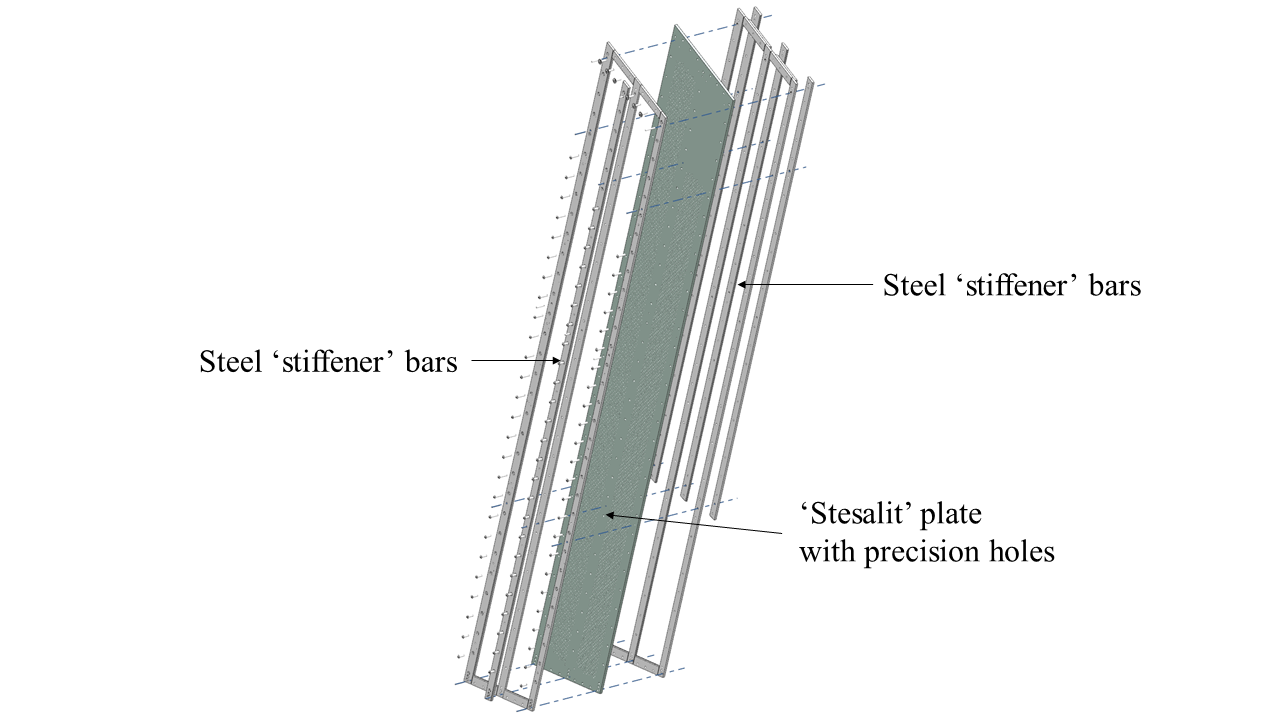
\includegraphics[width=0.5\columnwidth,natwidth=610,natheight=642]{img/dcr2-endplate.png}}}
\end{picture}
\caption{\small{A R2 endplate assembly.}}
\label{dcr2-endplate}
\end{figure}   
%%%%%%%%%%%%%%%%%%%%%%%%%%%%%%%%%%%%%%%%%%%%%%%%%%%%%%%%%%%%%%%%%%%%%%%%%%

It also allows 
the trumpets that position the wires to be essentially flush with the endplates, 
rather than having to insulate the trumpets from the conducting endplates as in 
the other two Regions (see Fig.~\ref{dc-corner}).  This reduced the thickness of 
the inactive region by 1 to 2~cm.




 



\subsection{Region Three Construction}

\hskip 0.15 in
The R3 chambers were designed and constructed at Jefferson Laboratory.  
They had the same general shape as the other chambers but were larger,
4 m on a side so the wires were as long as 4 m.
To reduce the gravitational sag of these very long wires we
strung them at 40 grams, twice the nominal tension of 20 grams.

%%%%%%%%%%%%%%%%%%% Figure : Region Three Cross Section %%%%%%%%%%%%%%%%%%
\begin{figure}[htpb]
\vspace{7.9cm}
\caption{\small{Assembly drawing of a R3 chambers showing the component
parts and highlighting the Carbon fiber tubes at the entrance face and
the carbon-foam composite plate at the exit, which supported the endplates
agains the wire tension.}}
\label{r3_cut}
\end{figure}
%%%%%%%%%%%%%%%%%%%%%%%%%%%%%%%%%%%%%%%%%%%%%%%%%%%%%%%%%%%%%%%%%%%%%%%%%%%

Because these are the final tracking chambers, multiple scattering
at the chamber entrance is not as important as multiple scattering that
occurs at a R1 or a R2 chamber, for example.  This allowed us to 
build a chamber in which the endplates were not supported only on
their ends.  At the entrance face we included 7 thin-walled Carbon
fiber tubes to span the gap and hold the endplates apart.  At the
exit face the endplates were coupled to a triangular carbon-foam-carbon
composite plate which similarly supported the wire tension.







